\chapter{Bevezetés} % Introduction
\label{ch:intro}

\section{Absztrakt}

A hipergráfok gyakran alkalmazott matematikai eszközök az informatika számos területén, így a szemantikus web, bioinformatika, szenzorhálózatok, adatbázisrendszerek, szociális hálózatok, gépi látás és egyéb területek számos megoldása épül rájuk.
Ezen feladatok vizsgálata során különösen hasznos lehet a hipergráfok, illetve halmazrendszerek vizualizációja. Vizualizáció során egyszerre merül fel igény a mögöttes struktúra tökéletes leképezésére, a könnyű értelmezhetőségre (így esztétikai metrikákra), az általános alkalmazhatóságra, gyors futásidőre, és - ezzel összefüggésben - a megjeleníthető adathalmaz méretének maximalizálására is, továbbá gyakran felmerül a dinamikus környezet - akár a struktúra, akár 
Mint látható, ez egy felettébb összetett problémát eredményez, amely megoldására számos módszer született már a szakterületi irodalomban, azonban ezek gyakran szenvednek egy - vagy több - tervezési elv sérülésétől, így egyik sem terjedt el a gyakorlatban.
Jelen dolgozatban különböző optimalizációs módszerek, illetve heurisztikák teljesítményét vizsgáljuk a fenti szempontok alapján, különös tekintettel az általános alkalmazhatóságra és helyes leképezésre.

\newpage

\section{A dolgozat felépítése}

Segítendő a szövegben való tájékozódást, ebben az alfejezetben részletezem a dolgozat felépítését. A diplomamunkára vonatkozó szabályoknak megfelelően három fejezetre bomlik a szöveg. Az első (Bevezetés című) fejezet további három nagyobb részre bontható. Az első ilyenben megadom a probléma leírásához, illetve megértéséhez szükséges definíciókat és fogalmakat, majd a tágabb és szűkebb problématerület irodalmi áttekintésére kerül sor, a probléma pontos megfogalmazásával lezárva. A második elkülönülő része a bevezetésnek a megoldás során alkalmazott módszereket, illetve az azokhoz közvetlenül kapcsolódó definíciókat írja le. A bevezetés végén a különböző megoldási módszerek teljesítményét vizsgáljuk, különböző hiperparaméterek mellett.


A mérések során alkalmazott szoftver felhasználói dokumentációját a második (Felhasználói dokumentáció), míg fejlesztői dokumentációját a harmadik (Fejlesztői dokumentáció című) fejezetében találhatjuk.

\begin{note}
A dolgozatban szereplő egyes szakszavak (néha egész szakterületek) egyáltalán nem, vagy nem elég hangsúlyosan szerepelnek a magyar szakirodalomban ahhoz, hogy elterjedt fordításuk legyen. Ezekben az esetekben - további figyelmeztetés nélkül - az angol nyelvű megfelelőjüket fogom használni. Népszerű, szinonímaként használt szakkifejezéseket igyekszem per jellel elválasztva felsorolni.
\end{note}

\section{Probléma}

\subsection{Alapdefiníciók}

Ahhoz, hogy megértsük a megoldandó problémát, számos fogalmat át kell tekintsünk először.

\subsubsection{Gráfok}

A gráf (variációi) alapvető fontosságú adattípus(ok) a modern informatikai megoldások során. Definiálásuk nem csak a dolgozat későbbi részeiben felbukkanó algoritmusok miatt fontos, hanem a - gyakran a gráfok általánosításának tekintett - hipergráfok mélyebb megértését is elősegítik. 

\begin{definition}
\textbf{Irányítatlan gráfnak} nevezünk egy olyan, rendezett $G=(V,E)$ párt, ahol $V$ egy nem-üres halmaz, $E$ pedig egy olyan multihalmaz, amely a $V$ elmeiből képzett kételemű halmazokat tartalmaz. Formálisan $E \subseteq \{\{u,v\} | u,v \in V\}$. A $V$ halmazt \textbf{csúcshalmaznak} is szokás nevezni, elemeit \textbf{csúcsoknak}, míg $E$-t az \textbf{élhalmaz}, elemeit pedig \textbf{él} névvel illetjük. Az élek által tartalmazott elemeket az adott él \textbf{végpontjainak} hívjuk. Két csúcs \textbf{szomszédos}, ha van olyan él $G$-ben, amely őket tartalmazza, míg egy csúcs \textbf{izolált}, ha egyetlen élnek sem végpontja.
\end{definition}

\begin{definition}
Az $e_i, e_j \in E, i \neq j$ éleket \textbf{párhuzamos éleknek} nevezzük, ha $e_i=e_j$. \textbf{Hurokélnek} egy olyan élet nevezünk, amely $\{v, v\}$ formájú, azaz a két végpontja azonos.
\end{definition}

\begin{definition}
Az $v \in V$ él \textbf{fokszámát} $d$-vel jelöljük, és $d=| \{ e | e \in E \land v \in e \}|$. A $G$ gráf \textbf{k-reguláris}, ha minden csúcsának fokszáma $k$.
\end{definition}

\begin{definition}
\textbf{Egyszerű gráf} egy olyan irányítatlan gráf, amelyben sem párhuzamos, sem hurokélek nincsenek jelen.
\end{definition}

\begin{definition}
Egy $G=(V,E)$ gráf \textbf{line graphja} alatt az $L(G)=(E, \{ \{ e_i, e_j \} | v \in V \land v \in e_i \land v \in e_j, i \neq j \})$ gráfot értjük.
\end{definition}

% TODO
% utak, séták
% elérhetőség
% (erős) összefüggés
% teljes gráf
% részgráf
% klikk / teljes részgráf

\subsubsection{Halmazrendszerek és hipergráfok}

Mint az absztraktban is említettem, halmazalapú adatreprezentációkkal, így hipergráfokkal és halmazrendszerekkel az informatika számos területén találkozhatunk. Az egyes problématerületek - sőt gyakran egy problématerületet vizsgáló különböző szakcikkek - azonban egymással konkuráló definíciókat alkalmaznak. Gyakran a halmazrendszerek szinonímájának tekintik a fogalmat, míg például - a szakterület egyik alapművének számító - Hypergraphs c. \cite{berge_hypergraphs_book} kötet mind az általunk használt - mindjárt megismertetett - definícióhoz, mind a halmazrendszer alapúhoz képest megszorításokat vezet be.

\begin{definition}
A $H$ halmaz \textbf{hatványhalmaza} $\mathcal{P}(H) = \{x | x \subseteq H\}$, azaz a $H$ halmaz összes részhalmazainak halmaza.
\end{definition}

\begin{definition}
A $H$ halmaz fölötti $\mathcal{F}$ \textbf{halmazrendszert} $\mathcal{F} \subseteq \mathcal{P}(H)$-ként definiáljuk.
\end{definition}

\begin{definition}
Ebben a dolgozatban \textbf{irányítatlan hipergráf} vagy egyszerűen hipergráf alatt egy olyan, rendezett $H=(V,E)$ párt értünk, ahol $V$ a \textbf{(hiper)csúcsok} nem-üres halmaza, míg $E$, a \textbf{hiperélek} halmaza, egy olyan multihalmaz, amelynek az elemei $\mathcal{P}(V) \setminus \emptyset$-ből kerülnek ki.
\end{definition}

\begin{note}
A hipergráf, úgy is ismertek, mint a gráfok általánosításai, ahol minden hiperél pontosan 2 elemet tartalmaz, azaz 2-reguláris. Egyrészről ez jól láthatóan függ a választott gráf-, és hipergráfdefinícióktól. Az itt használt definíciók alapján hipergráfok nem tartalmazhatnak hurokéleket, viszont párhuzamos éleket igen, így nem tökéletes általánosításai az irányítatlan gráfoknak, viszont irányítatlan egyszerű gráfoknak már igen.
\end{note}

\begin{note}
Egy másik felmerülő kérdés a hipergráfok kapcsán a hiperutak, más szóval a tranzitivitás fogalma a hiperélek között. A szakirodalomban erre is több, azonban jobban elkülönülő definíció létezik. Az itt bemutatott eredmények nem építenek a tranzitív relációra, így tetszőleges definíció tételezhető fel.
\end{note}

\subsubsection{Gráf- és hipergráf-adatszerkezetek}

Gráfok gépi kezelésére köztes gráfreprezentációkra, gráfadatszerkezetekre van szükség. Leggyakrabban az adjacencia mátrix, az incidencia mátrix, az éllista és a ritka reprezentációk általános osztálya használatos. Mivel a megoldások során csak az első kettőt alkalmazzuk, ezért a többit itt nem is definiáljuk.

\begin{definition}
A $G=(V,E)$ gráf \textbf{adjacencia mátrixa} alatt azt a $|V| \times |V|$ méretű $A_G$ mátrixot értjük, amelyben $a_ij=1$, ha $\{v_i, v_j\} \in E$ és 0 egyébként.
\end{definition}

\begin{definition}
A $G=(V,E)$ gráf \textbf{incidencia mátrixa} alatt azt a $|V| \times |E|$ méretű $I_G$ mátrixot értjük, amelyben $i_jk=1$, ha $v_j \in e_k$ és 0 egyébként.
\end{definition}

\begin{definition}
A $H=(V,E)$ hipergráf \textbf{incidencia mátrixát} ugyanúgy definiáljuk, ahogy a gráfokon definált megfelelőjét.
\end{definition}

\begin{note}
Hipergráfok esetében az adjacencia mátrix nem értelmezett, azonban a szakirodalomban gyakran használnak gráfokat köztes reprezentációként, így különösen a bipartite incidence structure, a multimodal/multi-layer/multiplex/multidimensional graph/network és a line/intersection graph fogalmaknak érdemes utánanéznie az ez iránt érdeklődő olvasónak.
\end{note}

\begin{definition}
A $H=(V,E)$ hipergráf \textbf{line/intersection graphja} az $L(H)=(E, \{ \{ e_i, e_j \} | v \in V \land e_i \cap e_j \neq \emptyset, i \neq j \})$ képlettel kapott egyszerű gráfot fedi. Jól látható, hogy ez általánosíta a gráfok esetében alkalmazott definíciónak.
\end{definition}

\begin{definition}
Egy irányítatlan $H=(V_H,E_H)$ hipergráf \textbf{(szuper)duálisa} az a $G=(V_G,E_G)$ egyszerű gráf, amelyben $V_G=\{X | X \subseteq E_H \land \exists v \in V_H : ((\forall e \in X: v \in e) \land (\forall e \notin X : v \notin e) \}$ és $E_G=\{\{X,Y\} | X,Y \subseteq E_H, X \neq Y \land \exists v \in V_H : (v \in X \land v \in Y)\}$
\end{definition}

\begin{note}
Figyeljük meg, hogy a szuperduálisban szereplő csúcsok száma exponenciális az eredeti csúcshalmaz tekintetében!
\end{note}

\subsection{Gráfok ábrázolása}

Mivel a gráfok gyakran használt, és könnyen konceptualizálható modellek, ezért a számítógépes vizsgálat mellett gyakran előnyös a felhasználó számára vizualizálni őket. Gráfok reprezentálhatók halmazokként, numerikusan (erre később látni fogunk példát), azonban ember-gép közreműködések során a leggyakrabban olyan képként szokás ábrázolni őket, melyeken a csúcsok körökként, az őket összekötő élek pedig egyenes (egyes esetekben akár görbe) vonalakként.
%\\
% TODO
% \begin{figure}[H]
% 	\centering
% 	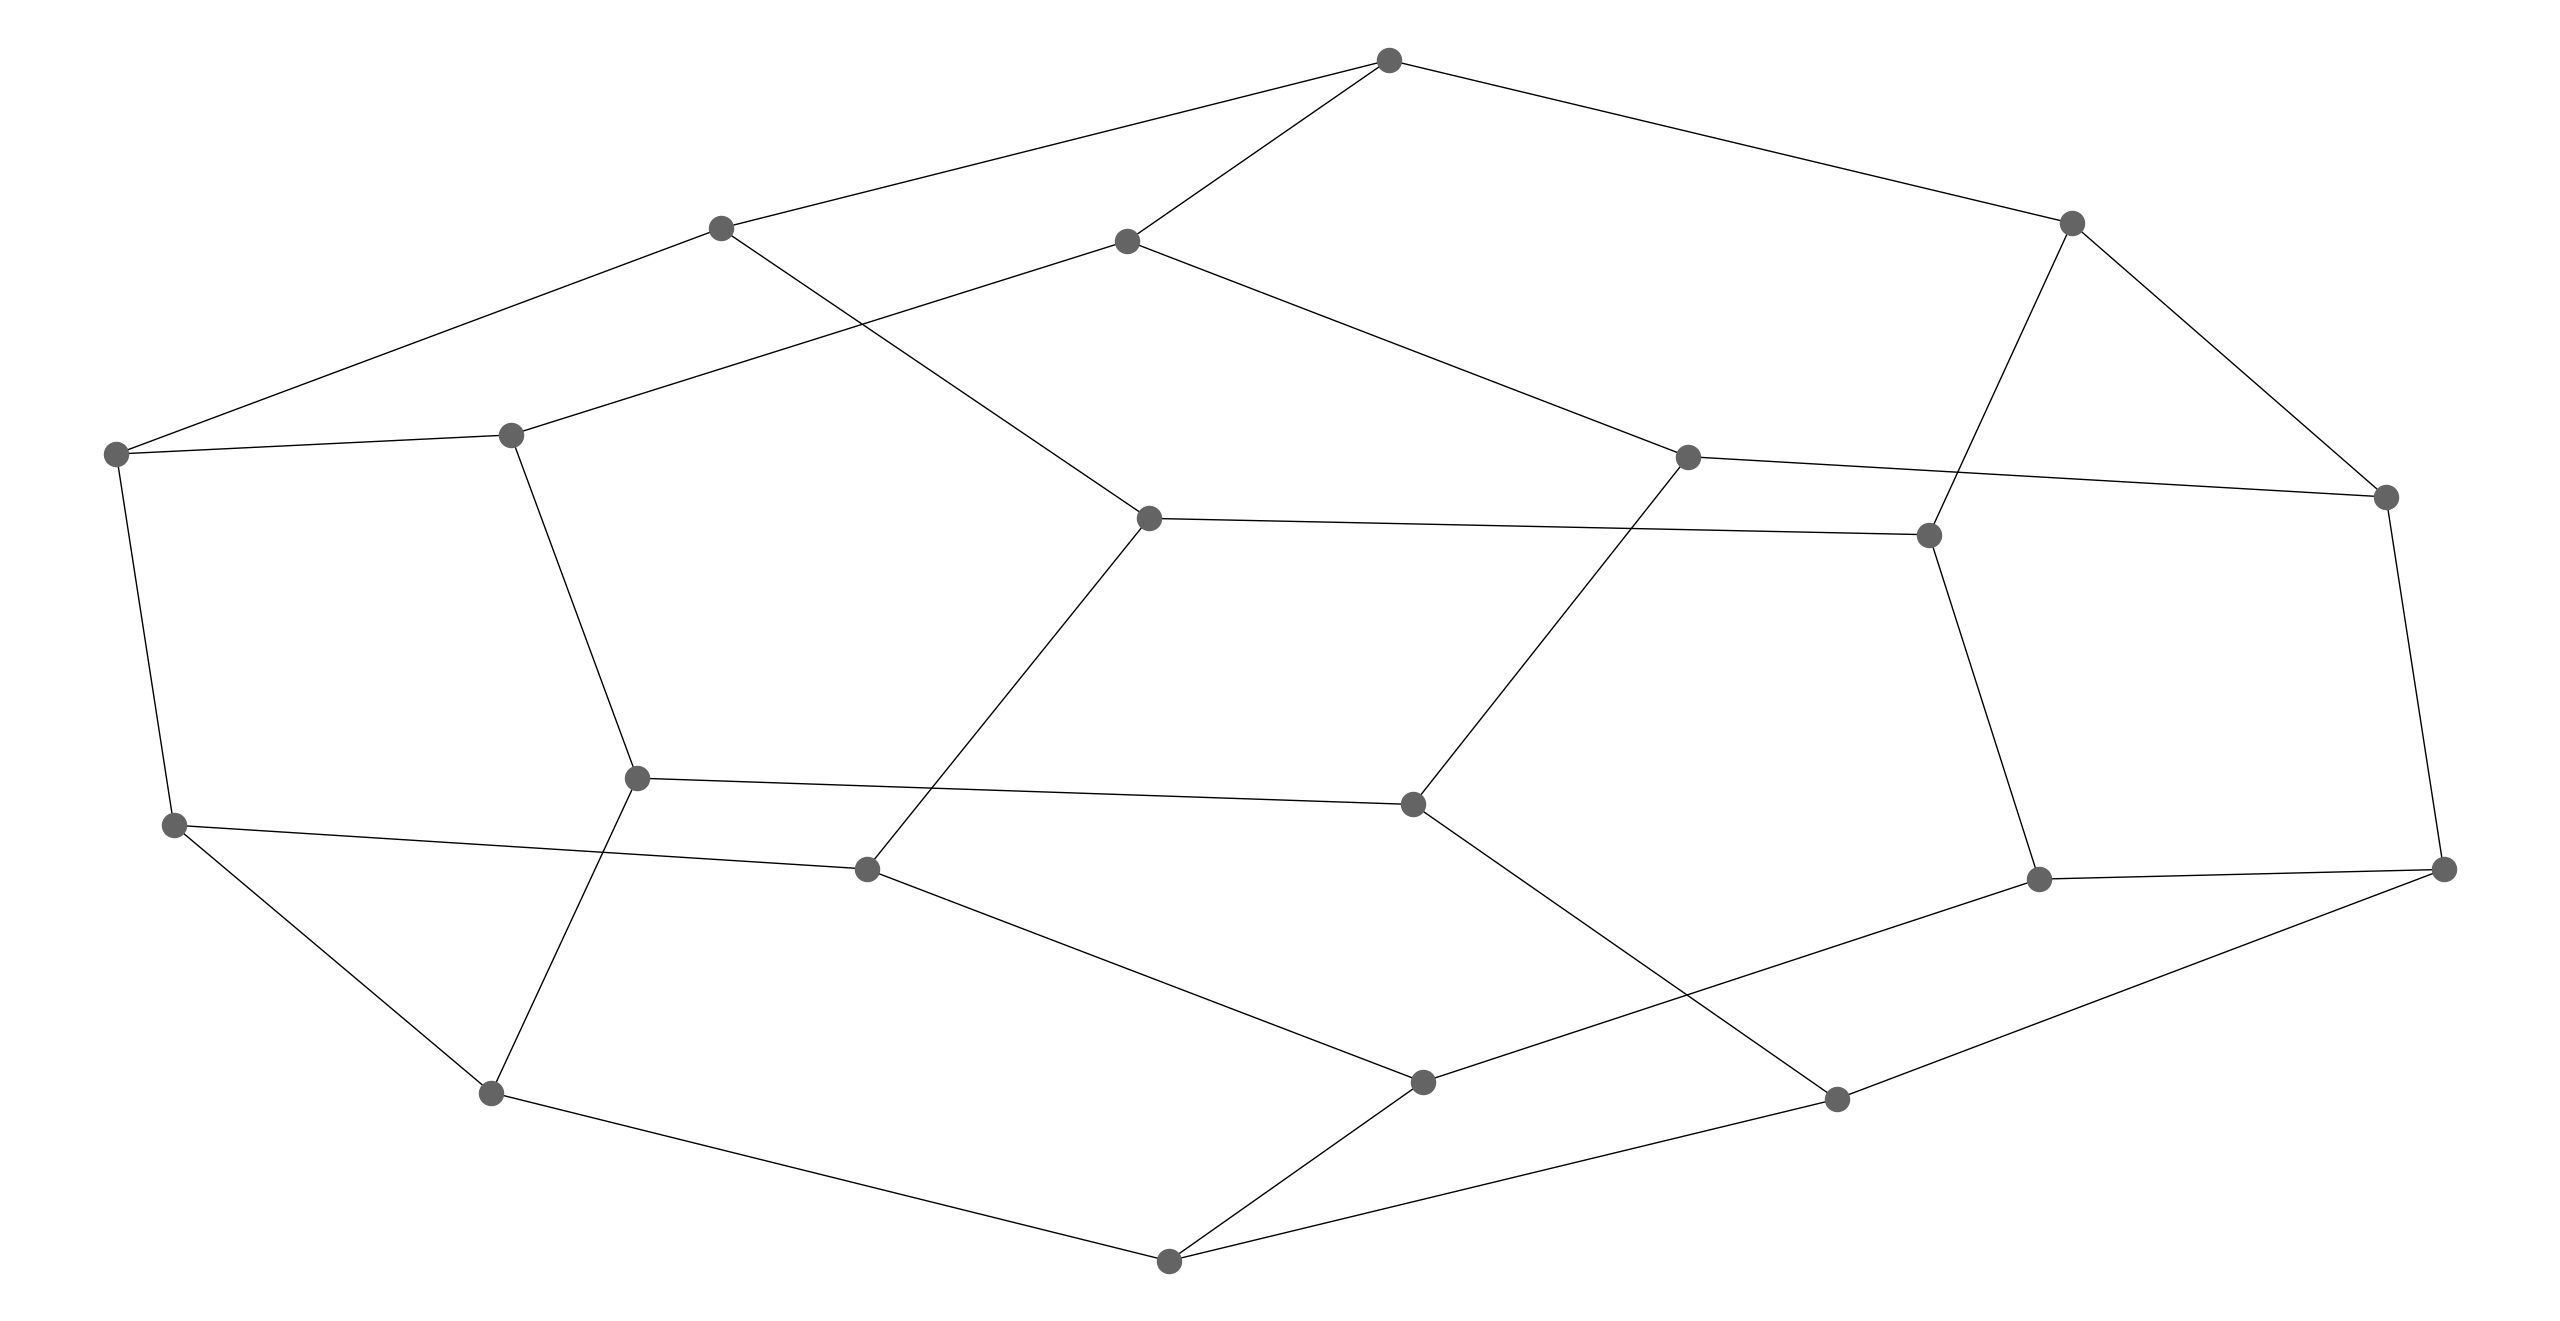
\includegraphics[height=100px]{simple_graph}
% 	\caption{Egyszerű gráf képi ábrázolása}
% \end{figure}

Gyakorlatban különösen fontos tulajdonságnak bizonyult - a könnyű értelmezhetőség szempontjából -, hogy egy adott gráf kirajzolható-e anélkül, hogy bármely két éle metszené egymást. A gráfelmélet egy ismert tétele, hogy nem minden gráf rajzolható síkba. A \textbf{Fáry-Wagner} tétel továbbá kimondja, hogy minden olyan gráf, ami görbe vonalak használatával síkbarajzolható, az egyenes vonalak esetén is síkbarajzolható marad.

\subsection{Hipergráfok és halmazrendszerek ábrázolása}

Gráfokhoz hasonlóan hipergráfok (és/vagy halmazrendszerek) esetén is hasznos a felhasználó által értelmezhető ábrázolásuk, azonban - a gráfoktól eltérő módon - a vizuális reprezentációjuk már egyáltalán nem egységes. A szakirodalom számos különböző módszert tart nyilván, melyeket Alsallakh és társai foglaltak össze\cite{alsallakah2016_the_state_of_the_art_set_visualization}. Az említett cikk számos különböző ábra kategóriát különböztet meg, én ezek közül kiemelném, hogy léteznek régiókon, vonalakon, mátrixokon és aggregáción alapuló, illetve hibrid módszerek. Az egyes kategóriák önmagukban is több ábrázolási módszert fednek, melyeket jellemzően egyenként is szakcikkek sokasága fed, így az áttekintésükre itt nincs módunk, azonban jól mutatja a kutatási terület mélységét.


Ebben a dolgozatban egy specifikus, régióalapú ábrázolási mód, az Euler-diagram vizsgálatát tűztem ki célul. Az Euler-diagram kirajzolását célzó algoritmusok az úgynevezett Euler Diagram Generation Problem (EDGP) megoldásai. Ahogy a neve is mutatja, a szóban forgó ábrázolási módot még maga Leonhard Euler vezette be a XVIII. században, azonban mindmáig előszeretettel használatos. Ahogy Baron írja\cite{euler_early}, Euler mindössze példákon mutatta be, illetve alkalmazta módszerét, nem definálta konkrétan. Ezek alapján - a hipergráfokhoz mintájára - Euler-diagramokra is többféle definíció létezik, melyek mind megyeznek abban, hogy az egyes halmazok/hiperélek zárt görbékkel reprezentáltak, melyek metszetei közös halmazelemeket feltételeznek, míg diszjunkt esetben azok hiányát. Egyes definíciók az alaphalmaz elemeit/hipercsúcsokat is elhelyezik az ábrán, így létrejöhetnek olyan metszetek is a vizualizáció során, melyek valójából üresek, de az értelmezés során ez mégsem okoz gondot. Gyakori kérdés, hogy a zárt görbék körök, ellipszisek vagy tetszőleges formájúak lehetnek-e, hogy szükségszerűen konvexek-e, illetve az egyes halmazok több, azonos címkével ellátott görbével is reprezentálhatók-e. A következőkben definiálom, hogy ebben a dolgozatban milyen értelmezést használok, azonban - az előzőeknek megfelelően - egyéb források ettől eltérhetnek.

\begin{definition}
A továbbiakban a $H=(V,E)$ hipergráfot reprezentáló \textbf{egyszerű Euler-diagram} alatt egy olyan ábrát értünk, amelyben minden $e \in E$ halmaz egyetlen zárt görbére képződik le, mely azokat, és csak azokat a hipercsúcsokat tartalmazza, melyek az adott $e$ hiperélnek is elemei. Azon hipercsúcsok, melyek egyetlen hiperélben sem szerepelnek, az összes görbén kívül kell megjelenjenek. Az egyes görbék címkével (esetünkben színekkel) rendelkeznek.
\end{definition}

% TODO
% \begin{figure}[H]
% 	\centering
% 	\includegraphics[height=100px]{euler_diagram}
% 	\caption{Példa egyszerű Euler-diagramra}
% \end{figure}

\begin{definition}
\textbf{Általánosított Euler-diagramként} vagy csak \textbf{Euler-diagramként} fogom nevezni azt az egyszerű Euler-diagramot, mely egy hiperélt több, azonos címkével ellátott zárt görbére is leképezhet.
\end{definition}

% TODO
% \begin{figure}[H]
% 	\centering
% 	\includegraphics[height=100px]{general_euler_diagram}
% 	\caption{Példa általánosított Euler-diagramra}
% \end{figure}

\subsection{Euler-diagramok vizualizációja}

\subsubsection{Síkbarajzolhatóság}

Gráfok esetében láthattuk, hogy felmerül a síkbarajzolhatóság kérdése. Amennyiben egyszer Euler-diagramokkal, így zárt, a végpontokat (jelen esetben hipercsúcsokat) tartalmazó görbékkel reprezentáljuk az éleket, akkor rögtön láthatjuk, hogy ezeknek tartalmazniuk kell legalább egy görbét is, amely közvetlenül összeköti a végpontokat. Ebből már észrevehetjük, hogy nem minden hipergráf rajzolható síkba egyszerű Euler-diagramokkal.


Verroust és Viaud bebizonyította\cite{drawability_8_sets}, hogy az általuk használt Euler-diagram definíció 8 halmazig megőrzi a síkbarajzolhatósági tulajdonságot. Simonetto és Auber egy másik struktúrát vizsgált\cite{simonetto_undrawable}, ami megfelel az itt általánosított Euler-diagramként definiált fogalomnak (ők Euler representationnek nevezik), melyről levezették, hogy alkalmas tetszőleges hipergráf síkbarajzolására. A szuperduális felhasználásával pontos leírása is adható annak, hogy mikor nem rajzolható ki egy hipergráf egyszerű Euler-diagramok használatával\cite{drawability_8_sets, simonetto_undrawable}. (Megjegyzendő, hogy a Sunibetto cikk intersection graphnak nevezi a szuperduálist, miközben az egy másik struktúrát jelöl, de a leírásból, illetve a példákból levezethető, hogy valójából felcserélték a kettőt.)

\subsubsection{Esztétikai mértékek}

Természetesen egy adott diagram síkbarajzolása nem feltétlenül szükséges ahhoz, hogy az ábra helyesen képezze le a mögöttes struktúrát (halmazrendszert vagy hipergráfot), azonban minenképpen megkönnyíti az emberi értelmezést. Egy adott ábra ilyen tulajdonságait esztétikai tulajdonságoknak nevezzük, ha pedig számszerűsíthetők (és adott rajtuk egy teljes rendezés), akkor esztétikai metrikáknak hívjuk. Esztétikai metrikák definiálhatók magukon a görbéken, a görbék metszetein, a csúcsok eloszlásán, az ábra színezésén, továbbá - gyakorlatilag - az ábrán megjelenő bármely aspektus fölött \cite{euler_force, which_well_formed, layout_metrics}.


Az EDGP során felmerülő két leggyakorabban vizsgált\cite{well_matchedness, euler_force, which_well_formed, orientation_comprehension} esztétikai tulajdonság, az úgynevezett well-formed és well-matched tulajdonságok.

\begin{definition}
Egy adott Euler-diagram esetén \textbf{kontúr/contour} névvel illetjük az egy címkéhez (vagy hiperélhez/halmazhoz) tartozó különböző zárt görbék összességét. \textbf{Minimális régiónak/minimal regionnek} hívjuk a görbék egymás által létrehozott legkisebb síkpartícióit, míg \textbf{alaprégió/basic region} alatt azon minimális régiók halmazát értjük, melyek ugyanazon görbék részei. Egy \textbf{zóna/zone} az alaprégiók egy olyan halmaza, amelyek azonos címkével rendelkeznek.
\end{definition}

A well-formed tulajdonság hat kritériumból tevődik össze, bár néha csak az első ötöt használják:

\begin{compactenum}
	\item Minden görbék egyszerű, azaz nem metszi önmagát - WFC1
	\item Nincs két görbe, amelynek közös határolószakasza van. (Az elfajuló, pontbeli találkozást nem vesszük hozzá - WFC2
	\item Nincs olyan pont, ahol három görbe érintkezik - WFC3
	\item Ha két görbe érintkezik, akkor metszik egymást - WFC4
	\item Minden zóna összefüggő, azaz egyetlen minimális régióból áll - WFC5
	\item Nem rendelkezik két görbe azonos címkével - WFC6\\
\end{compactenum}

A well-matched tulajdonság az alábbi négy tulajdonság meglétét fedi:

\begin{compactenum}
	\item Egy Euler-diagram well-matched a zónák szintjén, ha nem tartalmaz üres zónákat. - WMP1
	\item Egy Euler-diagram well-matched a görbék szintjén, ha a halmazok közti részhalmaz, metszet és diszjunkt relációk megfelelnek az adott halmazokat reprezentáló görbék tartalmazás, átfedés és diszjunkt tulajdonságának. - WMP2
	\item Egy Euler-diagram well-matched a minimális régiók szintjén, ha well-matched a zónák szintjén, és csak összefüggő zónákat tartalmaz. - WMP3
	\item Egy Euler-diagram well-matched a kontúrok szintjén, ha a halmazok közti részhalmaz, metszet és diszjunkt relációk megfelelnek az adott halmazokat reprezentáló kontúrok tartalmazás, átfedés és diszjunkt tulajdonságának. - WMP4\\
\end{compactenum}

Szintúgy széles körben vizsgált tulajdonság az area-proportionality, avagy méretarányosság\cite{euler_with_circles, area_proportional_phd, drawing_area_proportional, general_area_proportional}, amely azt mondja ki, hogy minden régió (bizonyos definíciók szerint az univerzumot reprezentáló kivételével) mérete úgy aránylik az ilyenek összegéhez, mint az $\omega$ súlyfüggvényük azok összegéhez. Leggyakrabban a zárt görbe által tartalmazott elemek számát alkalmazzuk súlyfüggvényként. Hibamértékek segítségével könnyen metrika is előállítható a tulajdonságból.

Annak ellenére, hogy több esztétikai metrika és tulajdonság is széles körben alkalmazott, nagyon kevés empirikus tapasztalatunk van arról, hogy ezek ténylegesen befolyásolják-e egy ábra értelmezhetőségét. Fish és társai kis mintán vizsgálták\cite{euler_comprehension} a well-formed tulajdonságnak az ábrák megértésére vonatkozó hatását. Az ő eredményeik alapján a WFC2 megsértése akár segítheti is egy ábra értelmezését, míg a WFC1 és WFC4 egyidejű, illetve a WFC3 vagy WFC4 önálló megsértése is rontja azt. Blake és társai\cite{orientation_comprehension} arra az eredményre jutottak, hogy az egyes görbék orientációja nincs hatással az emberi percepciójukra. Blake-ék egy másik cikkükben\cite{shape_comprehension} a szimmetrikus alakzatokat azonosították a legkönnyebben megérthetőként, így különösen a kör alakú reprezentációt javasolják.
%TODO cite colors - az IMDB-s cikknek van még egy érdekes color paragrafusa
%TODO alsakallah/CSR*14 - well matched fontosabb, mint well formed

\subsubsection{Euler-diagramok generálása}

Még úgy is, hogy az Euler-diagramok mindössze részterületét képezik a halmazábrázolási módszereknek, a szakirodalomban rengeteg különböző eljárás található, melyek gyakran nem is tekinthetők ugyanannak a szűken vett probléma megoldásának. Az alkalmazott Euler-diagram definíció, a vizsgált probléma mérete, az alkalmazott esztétikai tulajdonságok és metrikák, illetve ezek erős vagy gyenge megkövetelése mind-mind új variánsait hozzák létre a - összefoglaló néven EDGP-nek nevezett - problémának.

A halmazábrázolási terület legátfogóbb összegzését Alsallakh és társai adták\cite{alsallakah2016_the_state_of_the_art_set_visualization}, melyben számos EDGP megoldás összehasonlítását is adták (lásd az első táblázatot a cikkükben). Itt számos szempont alapján kategorizálják az egyes módszereket. Elsősorban megkülönböztetik a tetszőleges relációk ábrázolására alkalmas, illetve az ebben a tekintetben korlátozott megoldásokat. Ettől nem függetlenül megadják, hogy milyen alakzatokkal reprezentál egy halmazt az adott módszer (kör, poligon vagy ellipszis), a cikkből azonban sajnos kimaradt, hogy ismert Bézier-görbe alapú megoldás is\cite{layout_metrics}. Másik szempontként hozzák fel a teljesített esztétikai tulajdonságokat, mint a well-formed, well-matched, area-proportional, szimmetrikus görbe tulajdonságokat és vizsgálják, hogy létrejönnek-e üres minimális régiók (az univerzumon kívül). Az általuk adott táblázat alapján továbbá azt tételezhetjük fel, hogy az egyes módszerek vagy három, vagy tetszőleges számú halmazra alkalmazhatók. Megfigyelhető, hogy ezutóbbi az alapján válik el, hogy az Euler-diagramok egy speciális esetét, a Venn-diagramokat vizsgálja-e egy adott cikk vagy az általános problémát. Amiről ezek alapján nem kapunk képet, hogy egyes módszerek csak 8 halmazig alkalmazhatók\cite{drawability_8_sets}, mivel ezek fölött már ismertek olyan példák\cite{simonetto_undrawable, inductive_euler, drawability_8_sets}, amelyek nem síkbarajzolhatók egyes Euler-diagram definíciók szerint. (A cikkben nem említett, de hasznos kiemelni, hogy egyes algoritmusok csak már meglévő diagramok esztétikai javítását szolgálják\cite{euler_force} vagy emberi beavatkozást igényelnek\cite{sketch_euler}.)

A dolgozat későbbi részeiben legfontosabbnak Flower, Rodgers és Mutton munkájára\cite{layout_metrics} fog bizonyulni, akik sztochasztikus optimalizációs módszereket, illetve metaheurisztikákat alkalmaztak Bézier-görbékkel reprezentált Euler-diagramokra, és akikkel részben hasonló megközelítést választottunk. Érdemes még megemlíteni Stapleton és társainak munkáját\cite{inductive_euler}, amelyben induktív módon generálnak well-formed euler diagramokat, mikor ez lehetséges, a többi esetben pedig a well-formed kritériumok megsértésével, a görbék önmetszésével érik el, hogy továbbra is szemantikailag helyes ábrát generáljanak. Különösen érdemes megfigyelni, hogy az általánosság ilyen szintű eléréséhez a duális gráf egy módosított verzióját használják, ami exponenciális futásidőt eredményez.

\subsection{Problémaleírás}

Láthattuk, hogy az EDGP egy összetett probléma, amely magában foglalja a konkrét ábrázolási mód (Euler-diagram definíció), a vizsgált esztétikai metrikák, az elfogadható futásidő és a megoldható problémaméret meghatározását is. Különösen fontos kitérni arra is, hogy egy adott probléma vizsgálata során nem feltétlenül egyféle szempont szeretnénk ábrázolási módot választani. Elképzelhető, hogy ugyanúgy szeretnénk az előforduló klasztereket vizsgálni, mint a leghosszabb utakat, melyek másféle elrendezést tételeznek fel.


Az általam kitűzött célt az egyetemen folyó egyik kutatás igényei szerint tűztem ki, ahol adatbázisrendszerek redundanciáját csökkentjük hipergráfmodellek segítségével. Az itt folyó napi munka során egy olyan eszközre támadt szükség, amely - a jelenleg elérhető programokkal szemben - képes több tucat éllel és akár több száz csúcsal bíró hipergráfot többféle esztétikai metrika szerint is kirajzolni, akár hosszabb futási idő (órák) és/vagy egyszeri, kifejezetten hosszú (napok, hetek) tanulási idő után. Különösképp megnehezíti a feladatot, hogy Alsallakh és társai - a halmazábrázolási módszereket áttekintő cikkükben\cite{alsallakah2016_the_state_of_the_art_set_visualization} - az Euler-diagramokat mindössze 10-20 halmazig tartják alkalmazhatónak. A tématerület bonyolultságának és mélységének megfelelően a dolgozat különböző módszerek vizsgálatáról szól, a végső eszközt még nem hivatott létrehozni.


Mint láthattuk, az általános megoldhatóság érdekében emberi beavatkozás, korlát nélküli paramétertér (például Bézier görbék kontrollpontjai\cite{layout_metrics}) vagy exponenciális futásidő\cite{inductive_euler} lehet szükséges. Mivel tetszőleges esztétikai metrika fölött az optimalizáció, így a legjobb Euler-diagram megtalálása is NP-nehéz, ezért ez egyáltalán nem meglepő. A megoldásom alapjaként választott Flower cikkel\cite{layout_metrics} szemben, az általam használt, bonyolultabb problématér (mind a hipergráf méretében, egy adott halmazt reprezentáló zárt görbék számában és ebből kifolyólag a költségfüggvényként alkalmazott heurisztikák nem-folytonos jellegében) felveti a modell egyszerűsítésének igényét, illetve újabb heurisztikák kidolgozásának szükségességét is.

% -------------------------------------------------------------------------------------

\section{Megoldás}

\subsection{Optimalizáció}

A matematikai optimalizáció célja egy adott $f: X \rightarrow \mathbb{R} $ valós értékű függvény globális minimum- vagy maximumhelyének megtalálása, ahol X tetszőleges halmaz lehet. Mivel az $f$ függvény negáltja segítségével maximalizációs problémák minimalizáliós problémákká vezethetők vissza (vagy fordítva), ezért a kettő feladatot azonosnak tekintjük. A továbbiakban - mikor nem jelzem az ellenkezőjét - minimalizálási problémát tételezek fel.

\begin{definition}
Az $f$ függvényt számos módon nevezik; minimalizálási problémák esetén \textbf{költség-/veszteségfüggvényként} vagy \textbf{objektívfüggvényként}, míg maximálizálási problémák esetében \textbf{utility} vagy \textbf{fitness functionként} ismerjük. Egyes szakterületeken (mint fizikában) egyéb nevek is ismertek. Ha az $f$ függvény a $g_i, i \in \mathbb{N}_0$ függvények átlagaként áll elő, akkor költségfüggvénynek hívjuk, a $g_i$ függvényeket pedig veszteségfüggvényeknek.
\end{definition}

\begin{definition}
Egy optimalizálási algoritmus paramétereit \textbf{hiperparamétereknek} nevezzük.
\end{definition}

Általánosságban beszélve az optimalizálási probléma NP-nehéz, azonban a költségfüggvényre tett megszorításokkal ez feloldható. A kidolgozott algoritmusok ezért különösen fontos, hogy milyen megszorítások mellett operálnak.

\subsubsection{Gradiensalapú optimalizáció}
Gradiens-, illetve deriváltalapú algoritmusok vagy a deriváltfüggvényt (Hesse-mátrixot) vagy a pontbeli (parciális) deriváltat alkalmazzák. Bár szigorúan véve az első- és másodikderivált-próba is ide tartozik, a gyakorlatban a vizsgált függvény pontos képlete jellemzően nem ismert, illetve a paraméterek és a lokális szélsőértékek nagy száma is ellehetetleníti ezt a féle megoldást. Ezzel szemben iteratív mószereket szokás használni, melyek egy megadott - általában véletlenszerű - kiindulópontból egy lokális minimumponthoz konvergálnak. Amennyiben a függvény konvex vagy a kiindulópont kellőképpen közel volt a globális minimumhoz, akkor a kapott lokális minimumhely globálisan is az lesz, azonban ez általában nem garantált. Az előzőeknek megfelelően sokszor elvárt tulajdonság a folytonos deriválhatóság is.


A gyakorlatban használt legtöbb iteratív algoritmus a gradiens leszálláson alapszik. Gradiens leszállás során egy tetszőleges $\theta_0$ kiindulópontot választunk, majd a $\theta_{i+1} = \theta_i - \alpha * \nabla f(\theta_i)$ szabály alapján kiválasztjuk a következő vizsgálandó pontot, ahol $\alpha$ egy hiperparaméter. Az iteráció addig folytatódik, míg a megállási feltétel (például felső korlát az iterációk számára, a lépésköz nagyságára vagy a gradiensre egy normájára) nem teljesül. Fontos tulajdonsága ennek az algoritmusnak, hogy túl nagynak megválasztva $\alpha$-t átugorhatunk minimumhelyeket, míg túl kicsire állításával a keresési időt növeljük meg. Számos módszer született ennek a hiányosságnak az áthidalására, így egyes variációk az iterációk számának növekedésének függvényében csökkentik $\alpha$-t vagy eltérő kiindulópontokból indítják újra a keresést. Bizonyos feltételek mellett az algoritmus garantáltan egy lokális minimumhelyhez konvergál\cite{gradient_convergence}.


A gradiensalapú módszerekkel rokon jegyeket mutat a - nem feltétlenül differenciálható, de konvex függvények esetében a alkalmazható - szubgradiensmódszer, illetve az általánosabban használható, lokális keresésen alapuló hegymászó algoritmus (hill climbing).

\subsubsection{Sztochasztikus algoritmusok}

Összefoglaló néven \textbf{sztochasztikus algoritmus} névvel illetjük azokat a módszereket, amelyek futásuk során valószínűségi változókat alkalmaznak. Ez a megközelítés gyakran használt, mikor a költségfüggvény nem alkalmas direkt optimalizációra, viszont megelégszünk közelítő megoldásokkal is. Szintúgy előnyös, mikor a keresési térben számos, globális minimumértékhez közel álló pont létezik. A gradiens leszállás során látott véletlen kezdőpont kiválasztását inputnak tekintjük, így az algoritmus alapverzióját nem tekintjük sztochasztikusnak, viszont - mint számos egyéb determinisztikus (nem sztochasztikus) algoritmusnak - vannak sztochasztikus variánsai. Ennek megfelelően fontos kiemelni, hogy az egyes optimalizációs módszereknek általában több variánsa is létezhet, melyek esetenként összemossák a kategóriákat. Ennek a szekciónak a további részében át fogjuk tekinteni azokat az algoritmusokat, amelyeknek szükséges az ismerete a továbbiakban, azonban néhol pont az itt bemutatott alapverziótól való eltérés lesz különösen érdekes.


A legismertebb ilyen variáns az úgynevezett \textbf{sztochasztikus gradiens leszállás} (SGD). Mikor az $f$ költségfüggvény több $f_i$ veszteségfüggvény átlagaként jön létre, azaz $f(x) = 1/n * \sum_{i=1}^{n} f_i(x)$ (például gépi tanulás során több mintaelemen alkalmazva ugyanazt a veszteségfüggvényt), akkor előfordul, hogy a gradiens leszállás során a mai számítógépek kapacitásához képest túl sok parciális deriváltat kéne kiértékelni. Az SGD ez úgy kerüli el, hogy a veszteségfüggvényeket egyesével értekeli ki, mindegyik kiértékelés után modósítva a paramétereket. Láthatóan ez nem ekvivalens a teljes költségfüggvény gradiensének használatával (csak közelíti azt), továbbá nagyban függ a kiértékelés sorrendjétől is, ezért a veszteségfüggvények sorrendje a kiértékelés során randomizált. Néha szintúgy SGD-nek nevezik a mini-batch gradient descent módszert, ami annyiban tér el az SGD-től, hogy a paraméterek módosítása során egyszerre $k$ darab veszteségfüggvény átlagát használjuk, ahol $k$ egy hiperparaméter.


Természetben lejátszódó folyamatok számos esetben optimalizációs módszerként is tekinthetők. Az ilyen adaptált optimalizációs technikákat összefoglaló néven \textbf{biologiailag inspirált} algoritmusoknak nevezzük. A természeti rendszerek komplexitásából fakadó modellezési bizonytalanság feloldását sokszor a sztochaszticitás bevezetésével érjük el, így - gyakorlatban - a legtöbb biológiailag inspirált optimalizációs algoritmus egyben sztochasztikus algoritmus is.


Egy ilyen, természet ihlette algoritmus, a természetes szelekción alapuló \textbf{genetikus algoritmus} (GA)\cite{genetic_algorithm, non_gradient_optimization}. A módszer mögötti megfontolás, hogy egy populáció életciklusa a új egyedek születéséből/halálából, az egyedek szaporodásából (így genetikai keveredéséből), illetve mutációkból tevődik össze, ahol a párosodás a gének előnyös jellegének $f$ függvénye. Az algoritmus célja, hogy ezt az $f$ fitness függvényt \textit{maximalizálja}, az életképes egyedek kombinációjával, illetve kis, véletlenszerű módosításokkal. Az algoritmus pszeudokódja alább látható, azonban nem térünk ki minden részletére.

\begin{algorithm}[H]
\caption{Genetikus algoritmus}
\label{alg:ga} 
\textbf{\underline{Function}} GA($populationSize, parentNumber, mutationRate$)
\begin{algorithmic}[1] % sorszámok megjelenítése minden n. sor előtt, most n = 1
\STATE $t = 0$
\STATE $population_t$ = generateFeasibleSolutions($populationSize$)
\STATE $fitnessValues$ = evaluateFitness($population_t$)
\STATE $bestFitness, bestPosition = updateBest(fitnessValues, \infty, population_t, bestPosition)$
\WHILE{megállási feltétel nem teljesült}
	\STATE $parents$ = selectFitnessProportionally($population_t, fitnessValues, parentNumber$)
	\STATE $children$ = recombine($parents$)
	\STATE $population_t$ = deleteLast($population_t, fitnessValues, |children|$)
	\STATE $population_{t+1} = population_t \cup children$
	\STATE $population_{t+1}$ = mutate($population_{t+1}, mutationRate$)
	\STATE $fitnessValues$ = evaluateFitness($population_{t+1}$)
	\STATE $bestFitness = updateBest(fitnessValues, bestFitness, population_{t+1}, bestPosition)$
	\STATE $t = t + 1$
\ENDWHILE
\STATE \textbf{return} $bestFitness, bestPosition$
\end{algorithmic}
\end{algorithm}


Ahol $generateFeasibleSolutions(n)$ $n$ darab megengedett megoldást generál, $evaluateFitness(population)$ kiértékeli az egyes egyedek fitness értékeit, $updateBest(newValues, oldBest, newPositions, oldPosition)$ az új értékek és pozíciók, illetve a korábbi legjobbak segítségével kiválasztja a legjobbat (maximumot és maximumhelyet), $selectFitnessProportionally(population, fitnessValues, num)$ a fitness értékek által implikált valószínűségi eloszlás szerint kiválaszt $num$ darab egyedet, $recombine(population)$ két elemenként egy új egyedet hoz létre, amely a szülei génállományán alapszik, $deleteLast(population, fitnessValues, num)$ törli a $num$ darab legrosszabb fitness értékkel bíró egyedet a populációból, $mutate(population, mutationRate)$ pedig a $mutationRate$ arányában megváltoztatja az egyedek génállományát. A megállási feltétel gyakran iterációs felső korlát vagy alsó korlát a legjobb fitness értékre.


A \textbf{particle swarm optimization} (PSO) egy másik biológiailag inspirált algoritmus, amely analóg módon működik egyes rajként együtt dolgozó állat- és rovarfajokkal\cite{non_gradient_optimization, pso, modified_pso}. A módszer alapelve, hogy különböző, részecskéknek nevezett, entitások pozícióiban értékeljük ki az $f$ költségfüggvényt. A részecskék haladási iránnyal és sebességgel rendelkeznek, amelyet minden iterációban úgy frissítünk, hogy - véletlenszerű mértékben - figyelembe vesszük magát az irányt/sebességet és a részecske által, illetve a globálisan talált eddigi legjobb pozíciót/értéket.

\begin{algorithm}[H]
\caption{Particle swarm initialization}
\label{alg:pso} 
\textbf{\underline{Function}} InitializePSO($S, lowerBounds, upperBounds$)
\begin{algorithmic}[1] % sorszámok megjelenítése minden n. sor előtt, most n = 1
\STATE $bestPosition_{global} = \infty$
\FOR{$i=1 \ldots S$}
	\STATE $particlePosition_i \sim U(lowerBounds, upperBounds)$
	\STATE $bestPosition_i = particlePosition_i$
	\STATE $velocityRange = |upperBounds-lowerBounds|$
	\STATE $velocity_i \sim U(-velocityRange, velocityRange)$
	\IF{$f(bestPosition_i) < f(bestPosition_{global})$}
		\STATE $bestPosition_{global} = bestPosition_i$
	\ENDIF
\ENDFOR
\STATE \textbf{return} $bestPosition_{global}, particlePosition_{1 \ldots S}, bestPosition_{1 \ldots S}, velocity_{1 \ldots S}$
\end{algorithmic}
\end{algorithm}

\begin{algorithm}[H]
\caption{Particle swarm optimization}
\label{alg:pso} 
\textbf{\underline{Function}} PSO($S, w, c_1, c_2, lowerBounds, upperBounds$)
\begin{algorithmic}[1] % sorszámok megjelenítése minden n. sor előtt, most n = 1
\STATE $bestPosition_{global}, particlePosition_{1 \ldots S}, bestPosition_{1 \ldots S}, velocity_{1 \ldots S} = InitializePSO(S, lowerBounds, upperBounds)$
\WHILE{megállási feltétel nem teljesült}
	\FOR{$i=1 \ldots S$}
		\STATE $random_1, random_2 \sim U([0,1]^{dim(lowerBounds)})$
		\STATE $velocity_i = w*velocity_i + c_1*random_1*(bestPosition_i-particlePosition_i) + c_2*random_2*(bestPosition_{global}-particlePosition_i)$
		\STATE $particlePosition_i = particlePosition_i + velocity_i$ % \alpha * velocity_i
		\IF{$f(particlePosition_i) < f(bestPosition_i)$}
			\STATE $bestPosition_i = particlePosition_i$
			\IF{$f(bestPosition_i) < f(bestPosition_{global})$}
				\STATE $bestPosition_{global} = bestPosition_i$
			\ENDIF
		\ENDIF
	\ENDFOR
\ENDWHILE
\STATE \textbf{return} $f(bestPosition_{global}), bestPosition_{global}$
\end{algorithmic}
\end{algorithm}

Ahogy látható algoritmus hiperparméterek segítségével adja meg a részecskék számát, illetve a módosítási szabály egyes tagjainak súlyát

\subsubsection{Egyéb optimalizációs módszerek}
Természetesen az áttekintett kategóriákat nem merítettük ki, számos további algoritmus és variáns áttekintésére a dolgozat keretei között nincsen lehetőségem, illetve számos további megszorítás és függvényosztály is ismert, amelyekre létezik optimalizációs algoritmus, mint például lineáris egyenlőtlenségrendszerek vagy diszkrét halmazok esetén.

\subsection{Függvényapproximáció}

A numerikus analízis - így például az optimalizáció - számos területén merül fel a (jellemzően valós értékű) matematikai függvények használatának az igénye. Mikor a vizsgált függvény túl komplex, nem mindenhol kiértékelhető, esetleg nem rendelkezik az elvárt tulajdonságokkal, akkor függvények egy meghatározott részhalmazából kiválaszthatunk egy rá legjobban illeszkedőt. Ezt az eljárást - mint az ezt vizsgáló szakterületet - \textbf{függvényapproximációnak} nevezzük. Mikor meghatározott pontokban várjuk csak el a legjobb illeszkedést, akkor görbék illesztéséről beszélünk.


Legyen $f = \left(\begin{smallmatrix}f_1 & \ldots & f_n\end{smallmatrix}\right)^\top, w \in \mathcal{R}^n$, ahol $f_i, i=1 \ldots n$ tetszőleges függvény lehet. Ekkor az $f(x, w)$ \textbf{linear function approximatornek} nevezzük, ha az lineáris súlyok $w$ vektorában (bár nem feltétlenül az az $x$ inputban), azaz $f(x,w) = w_1*f_1(x) + \ldots + w_n*f_n(x)$. Mikor az $f$ függvény nem teljesíti a linearitási feltételt, akkor \textbf{nonlinear function approximatorről} beszélünk.

%TODO \subsubsection{Neurális hálók}


\subsection{Mély tanulás}
%TODO áttekintés
\subsubsection{Tanulás}
%TODO tanulás módja (inicializálás, batch, update, forward/backward propagation)
%(TODO regularizáció)
%TODO neuroevolution (-cikkek)
\subsubsection{Architektúrák}

% TODO ma

\subsection{Gráf konvolúciós neurális hálózatok}
%TODO áttekintés (jellemzően shallow, a bigyókára használatos, ahol vannak címkézett mintáink, és a a többi csúcsra szeretnénk általánosítani)
%TODO képlet
\subsubsection{Laplacian}
%TODO Laplacian
\subsubsection{Hipergráf Laplacian}
%TODO hypergraph laplacian - cikkek (random X hiányosságai!)
\subsubsection{Hipergráf konvolúciós neurális hálózatok}
%TODO áttekintés, hasonlóság a gráfokhoz, nehézségek (új hypergraph laplacian definíció)
%TODO képlet

%TODO holnap

\subsection{Alkalmazott Euler-diagram reprezentáció}
\subsection{Vizsgált optimalizációs módszerek}
% TODO GA variánsok (alg)
\subsection{Vizsgált inicializációs módszerek}

% TODO 27-én

% force directed
\subsection{Vizsgált heurisztikák}
\subsubsection{Szemantikus heurisztikák}
\subsubsection{Esztétikai heurisztikák}
\subsubsection{Futásidő analízis}


% TODO 28-án
%TODO színek problémája (cikkek), megoldása (rgb, hsv, genetic alg)

% -------------------------------------------------------------------------------------

\section{Mérések és következtetések}

%TODO 28-30 között
